\documentclass[twoside]{book}

% Packages required by doxygen
\usepackage{fixltx2e}
\usepackage{calc}
\usepackage{doxygen}
\usepackage[export]{adjustbox} % also loads graphicx
\usepackage{graphicx}
\usepackage[utf8]{inputenc}
\usepackage{makeidx}
\usepackage{multicol}
\usepackage{multirow}
\PassOptionsToPackage{warn}{textcomp}
\usepackage{textcomp}
\usepackage[nointegrals]{wasysym}
\usepackage[table]{xcolor}

% Font selection
\usepackage[T1]{fontenc}
\usepackage[scaled=.90]{helvet}
\usepackage{courier}
\usepackage{amssymb}
\usepackage{sectsty}
\renewcommand{\familydefault}{\sfdefault}
\allsectionsfont{%
  \fontseries{bc}\selectfont%
  \color{darkgray}%
}
\renewcommand{\DoxyLabelFont}{%
  \fontseries{bc}\selectfont%
  \color{darkgray}%
}
\newcommand{\+}{\discretionary{\mbox{\scriptsize$\hookleftarrow$}}{}{}}

% Page & text layout
\usepackage{geometry}
\geometry{%
  a4paper,%
  top=2.5cm,%
  bottom=2.5cm,%
  left=2.5cm,%
  right=2.5cm%
}
\tolerance=750
\hfuzz=15pt
\hbadness=750
\setlength{\emergencystretch}{15pt}
\setlength{\parindent}{0cm}
\setlength{\parskip}{3ex plus 2ex minus 2ex}
\makeatletter
\renewcommand{\paragraph}{%
  \@startsection{paragraph}{4}{0ex}{-1.0ex}{1.0ex}{%
    \normalfont\normalsize\bfseries\SS@parafont%
  }%
}
\renewcommand{\subparagraph}{%
  \@startsection{subparagraph}{5}{0ex}{-1.0ex}{1.0ex}{%
    \normalfont\normalsize\bfseries\SS@subparafont%
  }%
}
\makeatother

% Headers & footers
\usepackage{fancyhdr}
\pagestyle{fancyplain}
\fancyhead[LE]{\fancyplain{}{\bfseries\thepage}}
\fancyhead[CE]{\fancyplain{}{}}
\fancyhead[RE]{\fancyplain{}{\bfseries\leftmark}}
\fancyhead[LO]{\fancyplain{}{\bfseries\rightmark}}
\fancyhead[CO]{\fancyplain{}{}}
\fancyhead[RO]{\fancyplain{}{\bfseries\thepage}}
\fancyfoot[LE]{\fancyplain{}{}}
\fancyfoot[CE]{\fancyplain{}{}}
\fancyfoot[RE]{\fancyplain{}{\bfseries\scriptsize 制作者 Doxygen }}
\fancyfoot[LO]{\fancyplain{}{\bfseries\scriptsize 制作者 Doxygen }}
\fancyfoot[CO]{\fancyplain{}{}}
\fancyfoot[RO]{\fancyplain{}{}}
\renewcommand{\footrulewidth}{0.4pt}
\renewcommand{\chaptermark}[1]{%
  \markboth{#1}{}%
}
\renewcommand{\sectionmark}[1]{%
  \markright{\thesection\ #1}%
}

% Indices & bibliography
\usepackage{natbib}
\usepackage[titles]{tocloft}
\setcounter{tocdepth}{3}
\setcounter{secnumdepth}{5}
\makeindex

% Hyperlinks (required, but should be loaded last)
\usepackage{ifpdf}
\ifpdf
  \usepackage[pdftex,pagebackref=true]{hyperref}
\else
  \usepackage[ps2pdf,pagebackref=true]{hyperref}
\fi
\hypersetup{%
  colorlinks=true,%
  linkcolor=blue,%
  citecolor=blue,%
  unicode%
}

% Custom commands
\newcommand{\clearemptydoublepage}{%
  \newpage{\pagestyle{empty}\cleardoublepage}%
}

\usepackage{caption}
\captionsetup{labelsep=space,justification=centering,font={bf},singlelinecheck=off,skip=4pt,position=top}

%===== C O N T E N T S =====

\begin{document}

% Titlepage & ToC
\hypersetup{pageanchor=false,
             bookmarksnumbered=true,
             pdfencoding=unicode
            }
\pagenumbering{alph}
\begin{titlepage}
\vspace*{7cm}
\begin{center}%
{\Large live555\+\_\+rtsp \\[1ex]\large 1.\+00 }\\
\vspace*{1cm}
{\large 制作者 Doxygen 1.8.13}\\
\end{center}
\end{titlepage}
\clearemptydoublepage
\pagenumbering{roman}
\tableofcontents
\clearemptydoublepage
\pagenumbering{arabic}
\hypersetup{pageanchor=true}

%--- Begin generated contents ---
\chapter{live555\+\_\+rtsp}
\label{md__r_e_a_d_m_e}
\Hypertarget{md__r_e_a_d_m_e}
\input{md__r_e_a_d_m_e}
\chapter{继承关系索引}
\section{类继承关系}
此继承关系列表按字典顺序粗略的排序\+: \begin{DoxyCompactList}
\item \contentsline{section}{B\+U\+F\+T\+Y\+PE}{\pageref{struct_b_u_f_t_y_p_e}}{}
\item \contentsline{section}{Device}{\pageref{class_device}}{}
\item \contentsline{section}{Encoder}{\pageref{struct_encoder}}{}
\item Framed\+Source\begin{DoxyCompactList}
\item \contentsline{section}{H264\+Framed\+Live\+Source}{\pageref{class_h264_framed_live_source}}{}
\end{DoxyCompactList}
\item On\+Demand\+Server\+Media\+Subsession\begin{DoxyCompactList}
\item \contentsline{section}{H264\+Live\+Video\+Server\+Media\+Subssion}{\pageref{class_h264_live_video_server_media_subssion}}{}
\end{DoxyCompactList}
\end{DoxyCompactList}

\chapter{类索引}
\section{类列表}
这里列出了所有类、结构、联合以及接口定义等,并附带简要说明\+:\begin{DoxyCompactList}
\item\contentsline{section}{\hyperlink{struct_b_u_f_t_y_p_e}{B\+U\+F\+T\+Y\+PE} }{\pageref{struct_b_u_f_t_y_p_e}}{}
\item\contentsline{section}{\hyperlink{class_device}{Device} }{\pageref{class_device}}{}
\item\contentsline{section}{\hyperlink{struct_encoder}{Encoder} }{\pageref{struct_encoder}}{}
\item\contentsline{section}{\hyperlink{class_h264_framed_live_source}{H264\+Framed\+Live\+Source} }{\pageref{class_h264_framed_live_source}}{}
\item\contentsline{section}{\hyperlink{class_h264_live_video_server_media_subssion}{H264\+Live\+Video\+Server\+Media\+Subssion} }{\pageref{class_h264_live_video_server_media_subssion}}{}
\end{DoxyCompactList}

\chapter{类说明}
\hypertarget{struct_b_u_f_t_y_p_e}{}\section{B\+U\+F\+T\+Y\+P\+E结构体 参考}
\label{struct_b_u_f_t_y_p_e}\index{B\+U\+F\+T\+Y\+PE@{B\+U\+F\+T\+Y\+PE}}
\subsection*{Public 属性}
\begin{DoxyCompactItemize}
\item 
\mbox{\Hypertarget{struct_b_u_f_t_y_p_e_a1ee3a3ea7c63917b6266757049f0e78d}\label{struct_b_u_f_t_y_p_e_a1ee3a3ea7c63917b6266757049f0e78d}} 
char $\ast$ {\bfseries start}
\item 
\mbox{\Hypertarget{struct_b_u_f_t_y_p_e_ac71d7979baae81ee2205e040cddb9675}\label{struct_b_u_f_t_y_p_e_ac71d7979baae81ee2205e040cddb9675}} 
int {\bfseries length}
\end{DoxyCompactItemize}


该结构体的文档由以下文件生成\+:\begin{DoxyCompactItemize}
\item 
encoder\+\_\+define.\+hh\end{DoxyCompactItemize}

\hypertarget{class_device}{}\section{Device类 参考}
\label{class_device}\index{Device@{Device}}


Device 的协作图\+:
\nopagebreak
\begin{figure}[H]
\begin{center}
\leavevmode
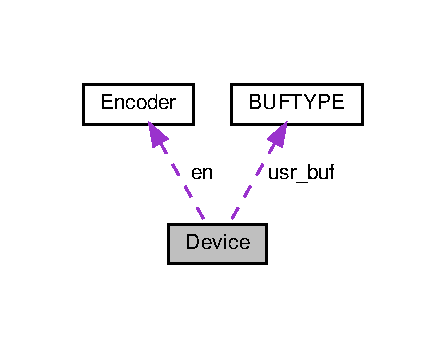
\includegraphics[width=214pt]{class_device__coll__graph}
\end{center}
\end{figure}
\subsection*{Public 成员函数}
\begin{DoxyCompactItemize}
\item 
\mbox{\Hypertarget{class_device_a177a1d7f5a34d87fd34f5dbaff9047cc}\label{class_device_a177a1d7f5a34d87fd34f5dbaff9047cc}} 
void \hyperlink{class_device_a177a1d7f5a34d87fd34f5dbaff9047cc}{init\+\_\+mmap} (void)
\begin{DoxyCompactList}\small\item\em 初始化摄像头内存映射 \end{DoxyCompactList}\item 
\mbox{\Hypertarget{class_device_a59fed87c831b9ca0087538041e1063fe}\label{class_device_a59fed87c831b9ca0087538041e1063fe}} 
void {\bfseries init\+\_\+camera} (void)
\item 
\mbox{\Hypertarget{class_device_ad733c28e25f18940a4b9c0f8c3bd5bbf}\label{class_device_ad733c28e25f18940a4b9c0f8c3bd5bbf}} 
void {\bfseries init\+\_\+encoder} (void)
\item 
\mbox{\Hypertarget{class_device_a207f256202dc6bcf3d431d7122a92027}\label{class_device_a207f256202dc6bcf3d431d7122a92027}} 
void {\bfseries open\+\_\+camera} (const char $\ast$devicename)
\item 
\mbox{\Hypertarget{class_device_a058dd0e33e2b9c9f7cd13e5e9c4d9e76}\label{class_device_a058dd0e33e2b9c9f7cd13e5e9c4d9e76}} 
void {\bfseries close\+\_\+camera} (void)
\item 
\mbox{\Hypertarget{class_device_a97b7011e07ec9d92f04aeaedfe6c1ae5}\label{class_device_a97b7011e07ec9d92f04aeaedfe6c1ae5}} 
void {\bfseries read\+\_\+one\+\_\+frame} (unsigned int \&framesize, unsigned char $\ast$f\+To)
\item 
\mbox{\Hypertarget{class_device_a57e890d08316be5b695f332e7ec833e7}\label{class_device_a57e890d08316be5b695f332e7ec833e7}} 
void {\bfseries getnextframe} (unsigned int \&framesize, unsigned char $\ast$f\+To)
\item 
\mbox{\Hypertarget{class_device_a91edaba797d1b176fd3077e6a2c85fe0}\label{class_device_a91edaba797d1b176fd3077e6a2c85fe0}} 
void {\bfseries start\+\_\+capture} (void)
\item 
\mbox{\Hypertarget{class_device_a760f2530ad1a3056ac13d7aaae9448f4}\label{class_device_a760f2530ad1a3056ac13d7aaae9448f4}} 
void {\bfseries stop\+\_\+capture} (void)
\item 
\mbox{\Hypertarget{class_device_a6fc123dd764c6fbda18eb69ea840a4e9}\label{class_device_a6fc123dd764c6fbda18eb69ea840a4e9}} 
void {\bfseries close\+\_\+encoder} ()
\item 
\mbox{\Hypertarget{class_device_a559094bf6961e9eba3712dc8591edca8}\label{class_device_a559094bf6961e9eba3712dc8591edca8}} 
int {\bfseries camera\+\_\+able\+\_\+read} (void)
\item 
\mbox{\Hypertarget{class_device_aaac3f374b03d0f56f280351d5f4465b4}\label{class_device_aaac3f374b03d0f56f280351d5f4465b4}} 
void {\bfseries compress\+\_\+begin} (\hyperlink{struct_encoder}{Encoder} $\ast$en, int width, int height)
\item 
\mbox{\Hypertarget{class_device_a6fbc13710308c3801e72a90ec3967a03}\label{class_device_a6fbc13710308c3801e72a90ec3967a03}} 
int {\bfseries compress\+\_\+frame} (\hyperlink{struct_encoder}{Encoder} $\ast$en, int type, char $\ast$in, int len, char $\ast$out)
\item 
\mbox{\Hypertarget{class_device_a811c381a9def366464189533b2a82130}\label{class_device_a811c381a9def366464189533b2a82130}} 
void {\bfseries compress\+\_\+end} (\hyperlink{struct_encoder}{Encoder} $\ast$en)
\item 
\mbox{\Hypertarget{class_device_a5a7aa55079fe5793415fbfc390de7c26}\label{class_device_a5a7aa55079fe5793415fbfc390de7c26}} 
void {\bfseries Init} (const char $\ast$devicename, int width, int height)
\item 
\mbox{\Hypertarget{class_device_a81e1f0d8a92771c4855d2831cfad77cc}\label{class_device_a81e1f0d8a92771c4855d2831cfad77cc}} 
void {\bfseries intoloop} ()
\item 
\mbox{\Hypertarget{class_device_a86bcc50a18a2ce9af12e97a7febb1651}\label{class_device_a86bcc50a18a2ce9af12e97a7febb1651}} 
void {\bfseries Destory} ()
\end{DoxyCompactItemize}
\subsection*{Public 属性}
\begin{DoxyCompactItemize}
\item 
\mbox{\Hypertarget{class_device_a471c31ce4b894f22afec70d1f1590782}\label{class_device_a471c31ce4b894f22afec70d1f1590782}} 
int {\bfseries fd}
\item 
\mbox{\Hypertarget{class_device_a3d152911845541f5446ee80a495b6f7c}\label{class_device_a3d152911845541f5446ee80a495b6f7c}} 
F\+I\+LE $\ast$ {\bfseries save\+\_\+fd}
\item 
\mbox{\Hypertarget{class_device_ab9d36e547656f839d6de58d7a32d2f3c}\label{class_device_ab9d36e547656f839d6de58d7a32d2f3c}} 
int {\bfseries n\+\_\+nal}
\item 
\mbox{\Hypertarget{class_device_a6feb7c01530f5a6da3591f879a288949}\label{class_device_a6feb7c01530f5a6da3591f879a288949}} 
int {\bfseries frame\+\_\+len}
\item 
\mbox{\Hypertarget{class_device_ac869882992a1eacf0b20c2626fc50297}\label{class_device_ac869882992a1eacf0b20c2626fc50297}} 
char $\ast$ {\bfseries h264\+\_\+buf}
\item 
\mbox{\Hypertarget{class_device_a38e039235792703a1d8dfc55856c89fd}\label{class_device_a38e039235792703a1d8dfc55856c89fd}} 
unsigned int {\bfseries n\+\_\+buffer}
\item 
\mbox{\Hypertarget{class_device_aaa76044ff91ebd8322df4050c782b8cb}\label{class_device_aaa76044ff91ebd8322df4050c782b8cb}} 
\hyperlink{struct_encoder}{Encoder} {\bfseries en}
\item 
\mbox{\Hypertarget{class_device_afb3ee5767b665069c4d092f958c5895a}\label{class_device_afb3ee5767b665069c4d092f958c5895a}} 
F\+I\+LE $\ast$ {\bfseries h264\+\_\+fp}
\item 
\mbox{\Hypertarget{class_device_a57193e929419148917d556eb6c7a912e}\label{class_device_a57193e929419148917d556eb6c7a912e}} 
\hyperlink{struct_b_u_f_t_y_p_e}{B\+U\+F\+T\+Y\+PE} $\ast$ {\bfseries usr\+\_\+buf}
\item 
\mbox{\Hypertarget{class_device_ad09954e6b78dabb3948a4fa9e5d08dfc}\label{class_device_ad09954e6b78dabb3948a4fa9e5d08dfc}} 
F\+I\+LE $\ast$ {\bfseries pipe\+\_\+fd}
\end{DoxyCompactItemize}


该类的文档由以下文件生成\+:\begin{DoxyCompactItemize}
\item 
camera.\+hh\item 
camera.\+cpp\end{DoxyCompactItemize}

\hypertarget{struct_encoder}{}\section{Encoder结构体 参考}
\label{struct_encoder}\index{Encoder@{Encoder}}
\subsection*{Public 属性}
\begin{DoxyCompactItemize}
\item 
\mbox{\Hypertarget{struct_encoder_a6844eefdfc8109863dff5db77988de75}\label{struct_encoder_a6844eefdfc8109863dff5db77988de75}} 
x264\+\_\+param\+\_\+t $\ast$ {\bfseries param}
\item 
\mbox{\Hypertarget{struct_encoder_af5a2b0d4bbbfecf57a4cd357cb8a9e8b}\label{struct_encoder_af5a2b0d4bbbfecf57a4cd357cb8a9e8b}} 
x264\+\_\+t $\ast$ {\bfseries handle}
\item 
\mbox{\Hypertarget{struct_encoder_a6b79affabf2ca3b4c3b71d79f9e61236}\label{struct_encoder_a6b79affabf2ca3b4c3b71d79f9e61236}} 
x264\+\_\+picture\+\_\+t $\ast$ {\bfseries picture}
\item 
\mbox{\Hypertarget{struct_encoder_aae78662ff4e865b3fa87a7e7c5f894c4}\label{struct_encoder_aae78662ff4e865b3fa87a7e7c5f894c4}} 
x264\+\_\+nal\+\_\+t $\ast$ {\bfseries nal}
\end{DoxyCompactItemize}


该结构体的文档由以下文件生成\+:\begin{DoxyCompactItemize}
\item 
encoder\+\_\+define.\+hh\end{DoxyCompactItemize}

\hypertarget{class_h264_framed_live_source}{}\section{H264\+Framed\+Live\+Source类 参考}
\label{class_h264_framed_live_source}\index{H264\+Framed\+Live\+Source@{H264\+Framed\+Live\+Source}}


类 H264\+Framed\+Live\+Source 继承关系图\+:
\nopagebreak
\begin{figure}[H]
\begin{center}
\leavevmode
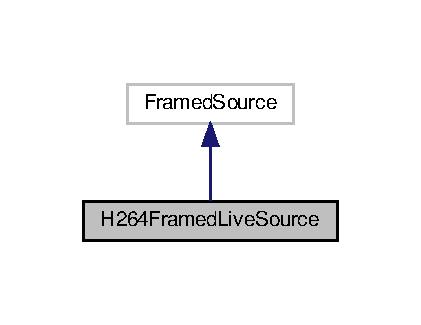
\includegraphics[width=202pt]{class_h264_framed_live_source__inherit__graph}
\end{center}
\end{figure}


H264\+Framed\+Live\+Source 的协作图\+:
\nopagebreak
\begin{figure}[H]
\begin{center}
\leavevmode
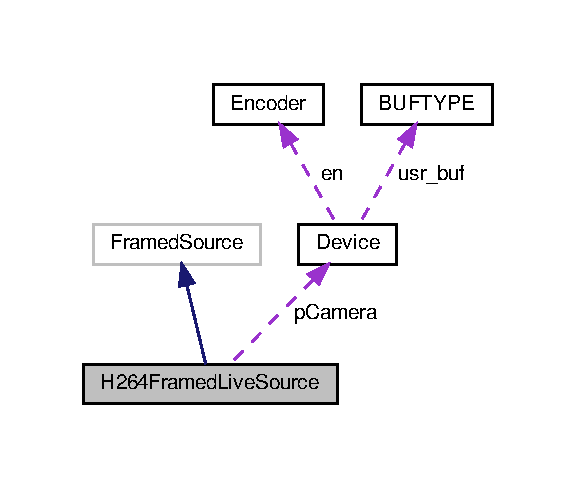
\includegraphics[width=277pt]{class_h264_framed_live_source__coll__graph}
\end{center}
\end{figure}
\subsection*{Public 成员函数}
\begin{DoxyCompactItemize}
\item 
\mbox{\Hypertarget{class_h264_framed_live_source_a5dcb3b51f285787f61818302367ce3d2}\label{class_h264_framed_live_source_a5dcb3b51f285787f61818302367ce3d2}} 
virtual unsigned {\bfseries max\+Frame\+Size} () const
\end{DoxyCompactItemize}
\subsection*{静态 Public 成员函数}
\begin{DoxyCompactItemize}
\item 
\mbox{\Hypertarget{class_h264_framed_live_source_a7c250dedd272ffc55b30c42e279228df}\label{class_h264_framed_live_source_a7c250dedd272ffc55b30c42e279228df}} 
static \hyperlink{class_h264_framed_live_source}{H264\+Framed\+Live\+Source} $\ast$ {\bfseries create\+New} (Usage\+Environment \&env, \hyperlink{class_device}{Device} $\ast$cam)
\end{DoxyCompactItemize}
\subsection*{Public 属性}
\begin{DoxyCompactItemize}
\item 
\mbox{\Hypertarget{class_h264_framed_live_source_a53b90d637797e98658148f524ac6499a}\label{class_h264_framed_live_source_a53b90d637797e98658148f524ac6499a}} 
class \hyperlink{class_device}{Device} $\ast$ {\bfseries p\+Camera}
\end{DoxyCompactItemize}
\subsection*{Protected 成员函数}
\begin{DoxyCompactItemize}
\item 
\mbox{\Hypertarget{class_h264_framed_live_source_afa33f8eb70b444565e68fdafa09ae43f}\label{class_h264_framed_live_source_afa33f8eb70b444565e68fdafa09ae43f}} 
{\bfseries H264\+Framed\+Live\+Source} (Usage\+Environment \&env, \hyperlink{class_device}{Device} $\ast$cam)
\end{DoxyCompactItemize}


该类的文档由以下文件生成\+:\begin{DoxyCompactItemize}
\item 
H264\+Framed\+Live\+Source.\+hh\item 
H264\+Framed\+Live\+Source.\+cpp\end{DoxyCompactItemize}

\hypertarget{class_h264_live_video_server_media_subssion}{}\section{H264\+Live\+Video\+Server\+Media\+Subssion类 参考}
\label{class_h264_live_video_server_media_subssion}\index{H264\+Live\+Video\+Server\+Media\+Subssion@{H264\+Live\+Video\+Server\+Media\+Subssion}}


类 H264\+Live\+Video\+Server\+Media\+Subssion 继承关系图\+:
\nopagebreak
\begin{figure}[H]
\begin{center}
\leavevmode
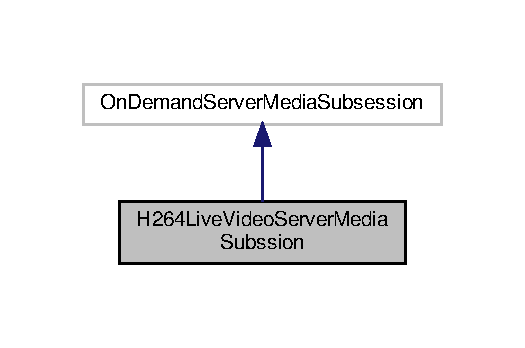
\includegraphics[width=252pt]{class_h264_live_video_server_media_subssion__inherit__graph}
\end{center}
\end{figure}


H264\+Live\+Video\+Server\+Media\+Subssion 的协作图\+:
\nopagebreak
\begin{figure}[H]
\begin{center}
\leavevmode
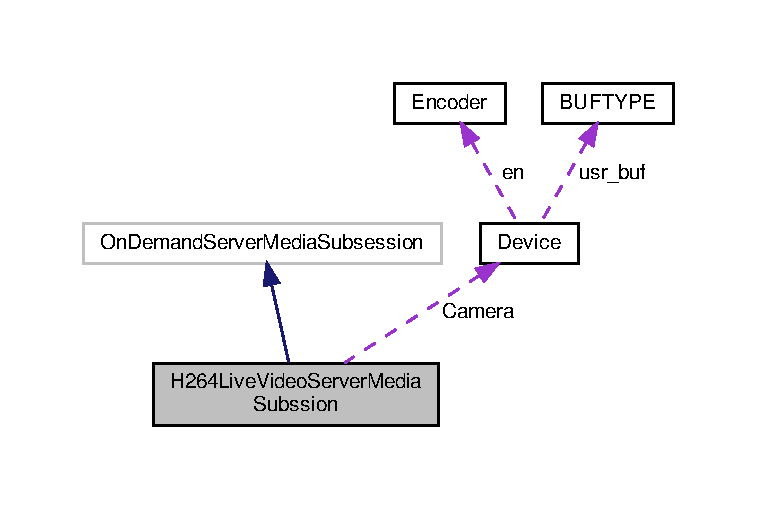
\includegraphics[width=350pt]{class_h264_live_video_server_media_subssion__coll__graph}
\end{center}
\end{figure}
\subsection*{静态 Public 成员函数}
\begin{DoxyCompactItemize}
\item 
\mbox{\Hypertarget{class_h264_live_video_server_media_subssion_a50d3d7bf02a7de9f7cf41a0a4f2238af}\label{class_h264_live_video_server_media_subssion_a50d3d7bf02a7de9f7cf41a0a4f2238af}} 
static \hyperlink{class_h264_live_video_server_media_subssion}{H264\+Live\+Video\+Server\+Media\+Subssion} $\ast$ {\bfseries create\+New} (Usage\+Environment \&env, Boolean reuse\+First\+Source, char const $\ast$devicename, int width, int height)
\end{DoxyCompactItemize}
\subsection*{Public 属性}
\begin{DoxyCompactItemize}
\item 
\mbox{\Hypertarget{class_h264_live_video_server_media_subssion_ad7052d7e26b215e97e17b53984cdbb67}\label{class_h264_live_video_server_media_subssion_ad7052d7e26b215e97e17b53984cdbb67}} 
class \hyperlink{class_device}{Device} {\bfseries Camera}
\end{DoxyCompactItemize}
\subsection*{Protected 成员函数}
\begin{DoxyCompactItemize}
\item 
\mbox{\Hypertarget{class_h264_live_video_server_media_subssion_abe88b44b0941148e9ee5269dfeb32f1e}\label{class_h264_live_video_server_media_subssion_abe88b44b0941148e9ee5269dfeb32f1e}} 
{\bfseries H264\+Live\+Video\+Server\+Media\+Subssion} (Usage\+Environment \&env, Boolean reuse\+First\+Source, char const $\ast$devicename, int width, int height)
\item 
\mbox{\Hypertarget{class_h264_live_video_server_media_subssion_aaca0b83b755639c5d903d05879936085}\label{class_h264_live_video_server_media_subssion_aaca0b83b755639c5d903d05879936085}} 
Framed\+Source $\ast$ {\bfseries create\+New\+Stream\+Source} (unsigned client\+Session\+Id, unsigned \&est\+Bitrate)
\item 
\mbox{\Hypertarget{class_h264_live_video_server_media_subssion_aa923aa0464fb45f2dba75866d2f22ead}\label{class_h264_live_video_server_media_subssion_aa923aa0464fb45f2dba75866d2f22ead}} 
R\+T\+P\+Sink $\ast$ {\bfseries create\+New\+R\+T\+P\+Sink} (Groupsock $\ast$rtp\+Groupsock, unsigned char rtp\+Payload\+Type\+If\+Dynamic, Framed\+Source $\ast$input\+Source)
\end{DoxyCompactItemize}


该类的文档由以下文件生成\+:\begin{DoxyCompactItemize}
\item 
H264\+Framed\+Live\+Source.\+hh\item 
H264\+Framed\+Live\+Source.\+cpp\end{DoxyCompactItemize}

%--- End generated contents ---

% Index
\backmatter
\newpage
\phantomsection
\clearemptydoublepage
\addcontentsline{toc}{chapter}{索引}
\printindex

\end{document}
